\section{Objectives}

\subsection{Main Objective}

The main objective of this project is to generate a black and white composite
video signal that will drive a Cathode Ray Tube (CRT) television. To accomplish
this, we will develop a video card with a serial interface that can generate a
composite video signal. We will be able to achieve a resolution of 240 x 320
pixels on the screen.

\begin{figure}[H]
   \centering
   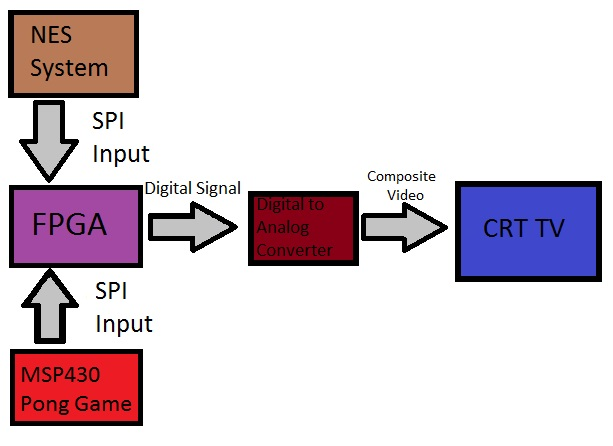
\includegraphics[scale=0.5]{Diagram.jpg}
   \caption{System Overview}
\end{figure}

\subsection{Secondary Objective}

\subsubsection{Colour}

The colour component of a composite signal is transmitted through the phase and
angle modulation of a 3.58MHz carrier. In order to generate this signal we would
need to employ a parallel DAC instead of our cheap, lopsided, but inexpensive
resistor divider DAC. Another project within our class is to create a Ninstendo
Entertainment System on an FPGA, and so we will base our colour output on the
NES.

\subsection{Hardware}

To be able to complete this project we will need more hardware than what we 
currently have. We have a MSP430 microcontroller, the FPGA board, and a mini
black and white TV. We need an 8-bit parallel, single channel DAC. We will use
the AD9748 from Analog Devices Inc. which can be ordered from Digikey, and we
will also need a breakout board for the 32-QFN package which can also be picked
up from Digikey. Any hardware we may need, such as parts for filtering will be
provided by us.
